\section{Evaluation}\label{sec:eval}
We use sample files from twenty different ad hoc data sources to
evaluate our overall inference algorithm and the different
approaches to probabilistic tokenization.
These data sources, many of which are published on the
web~\cite{padsweb}, are mostly system-generated log files of various
kinds and a few ASCII spreadsheets describing business transactions.
The size of these input files ranges from a few dozen lines to a few
thousand.

To test a given tokenization approach on a particular sample file, we
first construct a statistical model using the given approach from the
other nineteen sample files.  We then use the resulting model to infer a
description for the selected file.  We repeat this process for all
three tokenization approaches (HMM, HMEM, and HSVM) and all twenty
sample files.  We use three metrics described in the following
sections to evaluate the results: {\em token accuracy},
{\em quality of description} and {\em execution time}.

\subsection{Token accuracy}
To evaluate tokenization accuracy for a model $M$ on a given sample
file, we compare the most likely sequence of tokens predicted by $M$,
denoted $S_m$, with the ideal token sequence, denoted $S$.  We define
$S$ to be the sequence of tokens generated by the hand-written \pads{}
description of the file.  We define three kinds of error rates, all
normalized by $|S|$, the total number of tokens in $S$:

\begin{eqnarray*}
\textrm{token error} & = & \frac{\textrm{number of misidentified tokens in $S_m$}}
    {|S|} \\[1ex]
\textrm{token group error} & = & \frac{\textrm{number of misidentified groups in $S_m$}}
    {|S|}\\[1ex]
\textrm{token boundary error} & = & \frac{\textrm{number of misidentified boundaries in $S_m$}}
    {|S|}
\end{eqnarray*}

\begin{table}[th]
\begin{center}
\begin{tabular}{|l||c|c|c|c||c|c|c|c||c|c|c|c|} \hline
Data source        & \multicolumn{4}{|c||}{Token Error (\%)} &
               \multicolumn{4}{|c||}{Token Group Error (\%)} &
               \multicolumn{4}{|c|}{Token Boundary Error (\%)} \\ \cline{2-13}
               & lex   & HMM   & HMEM  & HSVM & lex & HMM & HMEM &
               HSVM & lex & HMM & HMEM & HSVM \\\hline\hline
1967Transactions     & 30    & 30    & 18.93 & 18.93 & 11.07 &
               11.07 & 0     & 0     & 11.07 & 11.07 & 0     & 0     \\ \hline
ai.3000              & 70.23 & 15.79 & 18.98 & 11.20 & 70.23 &
               14.68 & 17.26 & 10.27 & 53.53 & 12.34 & 4.79  & 4.00  \\ \hline
yum.txt                    & 19.44 & 13.33 & 21.80 & 0     & 19.17 &
               11.73 & 21.80 & 0     & 19.17 & 11.49 & 21.80 & 0     \\ \hline
rpmpkgs.txt                & 99.66   & 2.71  & 15.01 & 0.34  & 99.66
&
               2.14  & 14.67     & 0     & 99.66 & 0.23  & 14.67     & 0     \\ \hline
railroad.txt               & 51.94 & 9.47  & 6.48  & 5.58     &
51.94 &
               9.36  & 5.93  & 5.58     & 46.08 & 8.77  & 5.41  & 5.58     \\ \hline
dibbler.1000               & 15.72 & 43.40     & 11.91     & 0.00 &
15.72 & 36.78
                     & 11.91     & 0.00     & 4.54  & 13.33 & 13.15     & 0.00     \\ \hline
asl.log                    & 89.92 & 98.91 & 8.94  & 5.83  & 89.63 &
               98.91 & 8.94  & 5.83  & 83.28 & 98.54 & 6.27  & 3.29  \\ \hline
scrollkeeper.log           & 18.58 & 28.48 & 18.67 & 9.86  & 18.58 &
               18.77 & 8.96  & 0.12  & 18.58  & 17.83 & 8.96  & 0.12  \\ \hline
page\_log                  & 77.72 & 15.29 & 0     & 7.52  & 72.76 &
               15.29 & 0     & 7.52  & 64.70 & 5.64  & 0     & 5.64  \\ \hline
MER\_T01\_01.csv           & 84.56 & 23.09 & 31.32 & 15.40     &
84.56 &
               23.09 & 31.22 & 15.40     & 84.56 & 7.71  & 13.20 & 0.02 \\ \hline
crashreporter          & 51.89 & 7.91     & 4.99  & 0.19  & 51.85 &
7.91
                     & 4.96  & 0.14  & 51.34 & 7.91     & 4.92  & 0.14  \\ \hline
ls-l.txt                   & 33.73 & 18.70 & 19.96 & 6.65  & 33.73 &
               18.23 & 19.96 & 6.65  & 19.70 & 7.45  & 19.76 & 6.45  \\ \hline
windowserver\_last     & 73.31 & 14.98 & 10.16 & 3.24  & 71.50 &
               14.98 & 10.07 & 3.15  & 69.18 & 11.16 & 8.05  & 3.14  \\ \hline
netstat-an                 & 13.89 & 17.83 & 9.61  & 9.01  & 12.51 &
               15.44 & 5.95  & 5.95  & 12.51 & 14.90 & 5.80  & 5.20  \\ \hline
boot.txt                   & 10.67 & 25.40 & 9.37  & 2.77  & 3.99 &
               25.10 & 9.14  & 2.43  & 3.34  & 14.48 & 8.27  & 1.69  \\ \hline
quarterlyincome    & 82.99 & 5.52  & 1.98  & 1.98     & 82.99 &
               4.22  & 1.53  & 1.54     & 77.53 & 1.54  & 1.53  & 1.54     \\ \hline
corald.log            & 84.86 & 100   & 5.67  & 3.02     & 83.11 &
               98.25 & 3.93  & 1.27     & 81.76 & 97.80 & 1.27  & 1.27     \\ \hline
coraldnssrv.log       & 91.04 & 18.17 & 10.64 & 5.23  & 91.04 &
               18.17 & 9.33  & 5.22  & 83.07 & 14.37 & 4.11  & 3.92  \\ \hline
probed.log            & 1.74  & 27.99 & 16.50 & 16.50 & 1.74  &
               27.99 & 16.50 & 16.50 & 1.75  & 27.98 & 16.42 & 16.42 \\ \hline
coralwebsrv.log       & 86.67 & 100   & 8.75  & 23.99 & 86.67 &
               100   & 8.75  & 23.99     & 81.90 & 98.33 & 8.75  & 23.81     \\
               \hline
\end{tabular}
\sk
\caption{Tokenization errors} \shrink 
\label{tab:error}
\end{center}
\end{table}
The token error rate measures the number of times a token appears in
$S$ but the same token does not appear in the same place in $S_m$.
A {\em token group} is a set of token types that have similar
feature vectors and hence are hard to distinguish, e.g.
{\tt hex string} and {\tt id} which both consist of alpha-numeric
characters. The token group error rate measures the percentage of 
token groups in $S$ that do not exist in $S_m$ at the same locations.
Correct identification of token group is more desirable than confusing
with unrelated token types.
\cut{%%%%%%%%%%%%%%%%%%%
To define the token group error rate, we must first explain token
groups.  Some tokens have feature vectors that make them difficult to
distinguish, for example, the tokens {\tt hex string} and {\tt id}
which both contain digits and alphabetic letters.  Intuitively, if the
model misclassifies a {\tt hex string} as an {\tt id}, it is doing
better than if it predicts an unrelated token, such as a {\tt date}.
Each token group collects tokens with similar feature vectures, so the
tokens {\tt hex string} and {\tt id} belong to the same token group,
but not {\tt date}.  
number of times the model predicts a token outside of the token group
in the corresponding position in $S$.  More concretely, it measures the number of times a
token from a particular token group appears in $S$ but no token from
the same group appears in the same location in $S_m$.  Note that by
definition the token group error rate will always be lower than the
token error rate.
}%%%%%%%%%%%
The {\em token boundary} error rate measures the number of times
there is a boundary between tokens in $S$ but no corresponding
boundary in $S_m$.  This relatively coarse measure is interesting
because boundaries are important to structure discovery. Even if the
tokens are incorrectly identified, if the boundaries are correct, the
correct structure can be still discovered.

\tblref{tab:error} lists the token error, token group error, and token
boundary error rates of the twenty benchmarks. The results from
the original \learnpads{} system are presented in columns marked by 
{\tt lex}. It is evident that the original system produces high
error rates for many same files, because the lexer was unable to
use overlapping tokens effectively. HMM relies heavily on the transition
probabilities which requires more training samples than we have.
Therefore it does not perform as well as HMEM and HSVM in general.
In the case of {\tt asl.log}, {\tt corald.log} and {\tt coralwebsrv.log},
HMM's failure to detect some punctuation characters causes the
entire token sequences to be misaligned and hence gives very high
error rates.

\cut{ %%%%%%%%%%%
The {\tt lex} column
represents the results for the original \learnpads{} system.
The error rates are
high for the original system because the ideal \pads{} descriptions are
written using new tokens not available in the original system.
{\bf kenny: it might not be a good idea to include the lex columns?
ksf: It certainly does not make sense to include the numbers if they
are measuring something so different.  Is it possible to run the
original system with a tokenization file containing the new tokens?
}
For every data source except {\tt probed.log}, the
statistical models, especially HMEM and HSVM, substantially decrease token errors.
{\bf ksf: this is meaningless unless we fix the lex column.  We should
add a more meaningful summary of the data in the table.}
}%%%%%%%%%%%%

\subsection{Quality of description}
We use the {\em Minimum Description Length Principle}
(MDL)~\cite{mdlbook} to quantitatively assess description quality.
This principle says that a useful measure of description quality is
the sum of the cost in bits of transmitting the description (the
type cost) and the cost in bits of transmitting the data
\textit{given the description} (the data cost).  In general, the
type cost measures the complexity of the description, while the data
cost measures how loosely a given description explains the data.
Increasing the type cost generally reduces the data cost, and
\textit{vice versa}. The objective is to minimize both.
\tblref{tab:complexity1} shows the
percentage changes in the two costs of intermediate descriptions learned by
the new algorithm before refinement phase over that of the original \learnpads{} system.

\begin{table}[th]
\begin{center}
\begin{tabular}{|l||c|c|c||c|c|c|}\hline
Data source & \multicolumn{3}{|c||}{Type Cost} & \multicolumn{3}{|c|}{Data Cost}\\ \cline{2-7} 
& HMM & HMEM & HSVM & HMM & HMEM & HSVM \\ \hline 
1967Transactions & -39.661 & -27.03 & -27.03 & -2.80 & -2.80 & -2.80  \\ \hline
ai.3000 & -26.27 & +4.44 & -19.27 & -3.16 & -6.85 & -12.68            \\ \hline
yum.txt & -57.60 & +50.93 & -76.27 & -1.55 & -7.93 & -1.05            \\ \hline
rpmpkgs.txt & -92.03 & -76.29 & -91.86 & +1.47 & -0.00 & +1.47        \\ \hline
railroad.txt & -31.86 & -20.88 & -22.93 & -29.54 & -29.22 & -29.16    \\ \hline
dibbler.1000 & +611.22 & +17.83 & +7.03 & -19.88 & -22.11 & -22.10    \\ \hline
asl.log & -75.71 & -22.33 & -25.54 & +8.57 & -15.13 & -17.53          \\ \hline
scrollkeeper.log & -14.55 & -58.86 & -21.18 & -7.77 & -9.98 & -11.36  \\ \hline
page\_log & 0 & 0 & 0 & -11.46 & -11.67 & -11.67                      \\ \hline
MER\_T01\_01.csv & -8.59 & -12.74 & -12.74 & -25.59 & -24.15 & -24.14 \\ \hline
crashreporter & +4.03 & -8.66 & -12.73 & -9.38 & -9.41 & -12.45       \\ \hline
ls-l.txt & -74.61 & -51.32 & -39.30 & +0.10 & -7.26 & -2.18           \\ \hline
windowserver\_last & -62.84 & -33.29 & -56.18 & +6.93 & -11.12 & -9.87 \\ \hline
netstat-an & +147.07 & -12.00 & -21.63 & +14.18 & +6.74 & +7.65       \\ \hline
boot.txt & -72.60 & -38.95 & -71.29 & +5.26 & -6.54 & -5.03           \\ \hline
quarterlyincome & -18.36 & -18.36 & -18.36 & -32.04 & -32.51 & -32.51 \\ \hline
corald.log & -4.75 & -5.53 & -5.53 & -27.28 & -29.81 & -29.81         \\ \hline
coraldnssrv.log  & -1.86 & -2.03 & -5.86 & +59.53 & +59.53 & +59.53   \\ \hline
probed.log & -14.61 & -33.48 & -33.48 & +59.53 & +63.18 & +63.18      \\ \hline
coralwebsrv.log & -8.75 & +94.58 & -71.55 & -49.30 & -15.91 & +13.36  \\ \hline
\end{tabular}
\sk
\caption{Increase (+\%) or decrease (-\%) in type cost and data
cost before refinement} \label{tab:complexity1} \shrink
\end{center}
\end{table}

We can see that for most of the data sources, the probablistic tokenization
scheme improved the quality of the description by reducing both the type and
the data costs. In a few exceptional cases, a few misidentified tokens in
{\tt dibbler.1000}, {\tt netstat-an} and {\tt coralwebsrv.log} cause the 
entire descriptions to be drastically different from the ones produced by
the original system.


\cut{%%%%%%%%%%%
\begin{table}[th]
\begin{center}
\begin{tabular}{|l||c|c|c||c|c|c|}\hline
Data source & \multicolumn{3}{|c||}{Type Cost} &
\multicolumn{3}{|c|}{Data Cost}\\ \cline{2-7} 
& HMM & HMEM & HSVM & HMM &
HMEM & HSVM \\ \hline 
1967Transactions 	& -6.33 & -6.33 & -6.33 & +3.01 & +3.01 & +3.01 \\ \hline 
ai.3000 		& -44.64 & -35.85 & -52.00 & +34.81 & +20.05 & +25.91 \\ \hline 
yum.txt 		& -81.66 & -76.41 & -84.37 & +57.57 & -52.70 & -70.02  \\ \hline 
rpmpkgs.txt 		& -93.94 & -99.08 & -87.54 & +32.42 & +32.93 & +32.39 \\ \hline 
railroad.txt 		& -81.4 & -65.12 & -71.10 & +47.74 & +48.67 & +49.53 \\ \hline
dibbler.1000 		& +177.60 & +180.90 & +6.40 & -27.46 & -0.22 & -0.13 \\ \hline 
asl.log 		& -89.66 & -23.68 & -23.96 & -76.44 & -10.86 & -13.16 \\ \hline 
scrollkeeper.log 	& -22.15 & +105.25 & +5.76 & +9.72 & -57.08 & +2.90 \\ \hline 
page\_log 		& +1.76 & +1.76 & +1.76 & 0 & 0 & 0 \\ \hline 
MER\_T01\_01.csv 	& -8.38 & -10.01 & -10.01 & -0.06 & +8.54 & +8.54 \\ \hline 
crashreporter 		& -61.48 & -8.37 & -26.57 & +573.61 & +11.51 & +19.50 \\ \hline 
ls-l.txt 		& -69.41 & -49.15 & -43.09 & +26.03 & +10.22 & +42.13 \\ \hline 
windowserver\_last 	& -76.75 & -60.52 & -83.20 & +73.91 & +3.39 & +9.30 \\ \hline 
netstat-an 		& -99.76 & -77.10 & -80.19 & +17.35 & +28.31 & +29.49 \\ \hline 
boot.txt 		& -96.55 & -86.66 & -91.16 & +49.50 & +32.54 & +47.95 \\ \hline 
quarterlyincome 	& +3.86 & +2.85 & +2.85 & -1.70 & -1.98 & -1.98    \\ \hline 
corald.log 		& +12.28 & +2.69 & +2.69 & -1.04 & -1.08 & -1.08   \\ \hline 
coraldnssrv.log  	& -5.27 & +89.91 & -5.98 & +28.91 & -35.50 & +43.90 \\ \hline
probed.log 		& -31.41 & -31.41 & -31.41 & +28.92 & +28.92 & +28.92 \\ \hline
coralwebsrv.log 	& -36.21 & +35.98 & -52.08 & -25.04 & -14.33 & +69.42 \\ \hline
\end{tabular}
\caption{Increase (+\%) or decrease (-\%) in type cost and data
cost: after refinement} \label{tab:complexity2}
\end{center}
\end{table}

In practise, better tokenization schemes usually result in simpler
descriptions (lower type costs), but looser fits (higher data
costs). This trend is more clear in \tblref{tab:complexity1}, because
in the refinement phase, rules are coded particularly in favor of
descriptions generated by original \learnpads{} system. \tblref{tab:complexity1} shows that in all benchmarks except
{\tt dibbler.1000}, {\tt coraldnssrv.log} and {\tt probed.log}, at
least one of the statistical models significantly reduces the type
cost while keeping the data cost stable.
}%%%%%%%%%%%%%
%This is not exactly consistent with the error rate
%evaluation, because even if most token sequences are correct, only a
%few wrong token sequences can cause a difference at the description
%level.

In another experiment, a human expert visually judged how each
description compared to the original \learnpads{} results. The
judgements focus on the readability of the descriptions, i.e.
whether the descriptions can present the structure of the data
sources clearly. In this experiment, the judge is asked to rate the
descriptions one by one, in a scale from -2 (meaning the description is
too concise and it loses much useful information) to 2 (meaning the
description is too precise and the structure is unclear). The
score of a good description is therefore close to 0, which means the
description provides sufficient information for the user to
understand the data source and meanwhile the user can easily tell
the structure from the description. \tblref{tab:expert} shows that
on average, HMEM and HSVM clearly outperforms the original system
denoted by {\tt lex}.

%Although the original \learnpads{}
%system is incapable of identifying tokens as well as \learnpads{} with
%statistical models, the structure discovery and refinement phases are
%still quite effective.
%The new \learnpads{} system doesn't rely on the refinement rules that much.
\cut{%%%%%%%%%%%%%%
For benchmarks where the original system produces good descriptions,
the new system outputs similarly good descriptions. For
data sources for which the original system did poorly,
the new system offers improvements.
{\bf kf This claim does not seem to be supported by the data in the
  table. }
}

\begin{table}[th]
\begin{center}
\begin{tabular}{|l|c|c|c|c||l|c|c|c|c||}\hline
Data source & lex & HMM & HMEM & HSVM & Data source & lex & HMM & HMEM & HSVM \\ \hline 
1967Transactions & 0& 0 & 0 & 0 &   crashreporter & 2 & 0 & 1 & 1 \\ \hline 
ai.3000 & 1 & 1 & 1 & 0   &         ls-l.txt & 2 & 0 & 1 & 1 \\ \hline 
yum.txt & 2 &  -1 & 1 & 0   &       windowserver\_last & 2 & 0 & 1 & 1 \\ \hline 
rpmpkgs.txt & 2 & -1 & -2 & 0 &     netstat-an & 2 & -2 & 0 & 0 \\ \hline 
railroad.txt & 2 & 1 & 1 & 1 &      boot.txt & 2 & -1 & 1 & 1 \\ \hline 
dibbler.1000 & 0 & 2 & 0 & 0 &      quarterlyincome & 1 & 1 & 1 & 1   \\ \hline 
asl.log & 2 & -2 & 2 & 2 &          corald.log & 0 & 1 & 1 & 0 \\ \hline 
scrollkeeper.log  &  1 & 2 & 1 & 1 &coraldnssrv.log  & 0 &  1 & 1 & -1 \\ \hline 
page\_log  & 0 & 0 & 0 & 0 &        probed.log & 0 & 0 & 0 & 0 \\ \hline 
MER\_T01\_01.csv & 0 & 1 & 0 & 0 &  coralwebsrv.log & 0 & 1 & 1 & -1 \\\hline
\end{tabular}
\sk
\caption{Qualitative comparison of descriptions learned using
probabilistic tokenization to descriptions learned by original \learnpads{} algorithm.}
\label{tab:expert}\shrink
\end{center}
\end{table}

%\begin{table}[th]
%\begin{center}
%\begin{tabular}{|l||c|c|c|}\hline
%Data source & HMM & HMEM & HSVM \\ \hline
%1967Transactions & no difference & no difference & no difference   \\\hline
%ai.3000 & better & better & better \\ \hline
%yum.txt & better &  better & better \\ \hline
%rpmpkgs.txt & better & better & better\\ \hline
%railroad.txt & slightly better & both complicated & both complicated  \\ \hline
%dibbler.1000 & slightly worse & not much difference & not much difference   \\ \hline
%asl.log & too concise & both complicated & both complicated \\ \hline
%scrollkeeper.log  &  better & better & better \\ \hline page\_log
%& slightly worse & not much difference & not much difference \\
%\hline MER\_T01\_01.csv & too concise & not much difference & not
%much difference \\ \hline crashreporter & slightly better & not much
%difference & better \\ \hline ls-l.txt & better & better & better \\
%\hline windowserver\_last & slightly better & slightly better &
%better \\ \hline netstat-an & better & better & better \\ \hline
%boot.txt & better &  better & better \\ \hline quarterlyincome &
%slightly better & slightly better & slightly better   \\ \hline
%corald.log & better &  better & better \\ \hline coraldnssrv.log  &
%not much difference &  not much difference & not much difference\\
%\hline probed.log & worse & not much difference & not much
%difference \\ \hline coralwebsrv.log & worse & worse & worse
%\\\hline
%\end{tabular}
%\caption{Qualitative comparison of descriptions learned using probabilistic
%  tokenization to descriptions learned by original \learnpads{}
%  algorithm.}
%\label{tab:expert}
%\end{center}
%\end{table}

\subsection{Execution time}

\begin{figure}[th]
\begin{minipage}[t]{0.4\columnwidth}
\begin{center}
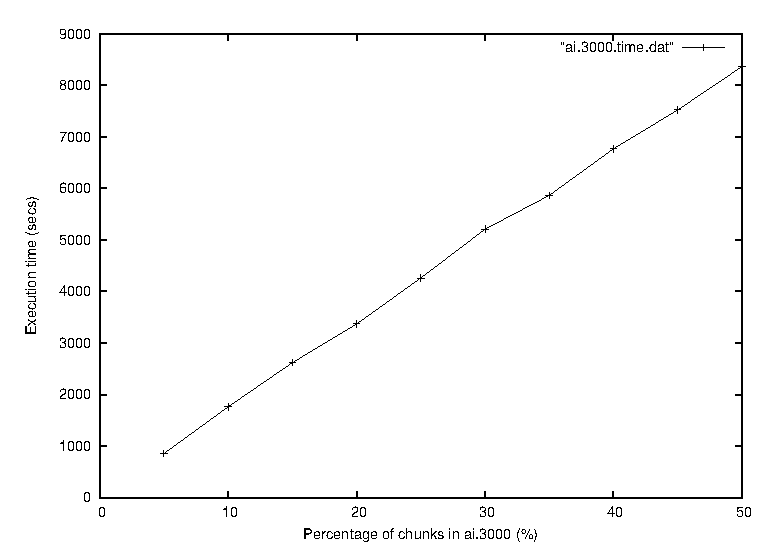
\epsfig{file=ai_1.eps, width=\columnwidth}
\end{center}
\caption{Execution time of ai.3000}\label{fig:ai_1}
\end{minipage}
\hfill
\begin{minipage}[t]{0.6\columnwidth}
\begin{center}
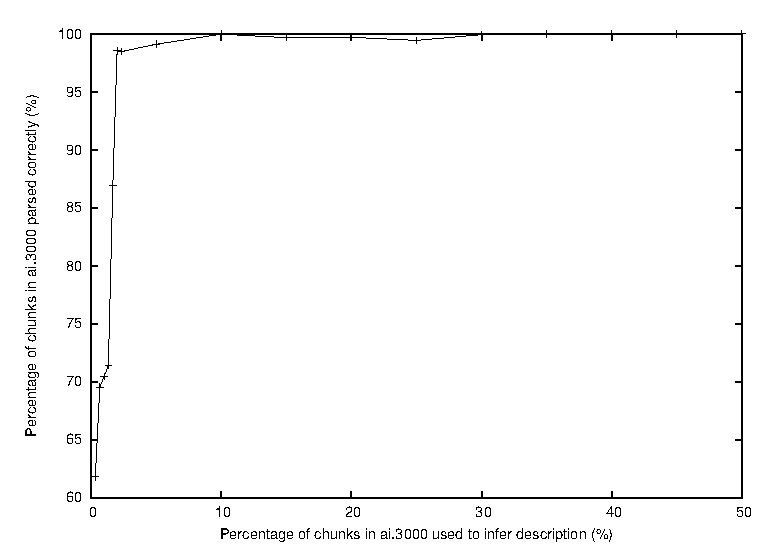
\epsfig{file=ai_2.eps, width=\columnwidth}
\end{center}
\caption{Success rates of ai.3000}\label{fig:ai_2}
\end{minipage}
\end{figure}
%\begin{table}[th]
%\begin{center}
%\begin{tabular}{|l||c|c|c|}\hline
%Data source & HMM & HMEM & HSVM \\ \hline
%1967Transactions & 72.96 & 678.373 & 1390.881   \\\hline
%ai.3000 & 1112.978 & 7565.64 & 27191.87 \\ \hline
%yum.txt & 47.381 &  819.373 & 835.01\\ \hline
%rpmpkgs.txt & 156.817 & 476.41 & 1489.92\\ \hline
%railroad.txt & 19.873 & 209.927 & 527.549  \\ \hline
%dibbler.1000 & 546.953 & 3431.927 & 5417.374   \\ \hline
%asl.log & 2021.906 & 14245.55 & 52296.55 \\ \hline
%scrollkeeper.log  &  50.062 & 565.278 & 1733.855 \\ \hline
%page\_log  & 23.69 & 312.321 & 999.72 \\ \hline
%MER\_T01\_01.csv & 10.931 & 351.63 & 516.667 \\ \hline
%crashreporter & 499.632 & 39.572 & 1849.967 \\ \hline
%ls-l.txt & 54.608 & 60.52 & 245.936 \\ \hline
%windowserver\_last & 276.393 & 1354.663 & 3685.615 \\ \hline
%netstat-an & 54.315 & 422.74 & 1192.808 \\ \hline
%boot.txt & 42.012 &  767.893 & 1547.052 \\ \hline
%quarterlyincome & 9.586 & 130.903 & 363.634   \\ \hline
%corald.log & 188.036 &  881.527 & 329.826 \\ \hline
%coraldnssrv.log  & 63.085 &  1553.705 & 6402.181\\ \hline
%probed.log & 298.278 & 1647.448 & 4433.592 \\ \hline
%coralwebsrv.log & 112.372 & 1175.747 & 4020.109 \\\hline
%\end{tabular}
%\caption{Time to produce inferred description in seconds}
%\label{tab:time}
%\end{center}
%\end{table}

Compared to the original system, 
statistical inference requires extra time to construct \seqset{}s and
compute probabilities. 
%\tblref{tab:time} summarizes the times required
%to produce inferred descriptions for the twenty data sources.
%{\bf kf: can we include a column for learnpads?}
We ran our experiments on a 2.2 GHz Intel Xeon processor with 5
GB of memory. The original algorithm takes anywhere from 
under 10 seconds to 25 minutes to infer a description, while the new system
requires a few seconds to several hours, depending on the amount of test data
and the statistical model used. In general, the character-by-character
HMM model is the fastest, while HSVM is most time-consuming.
%Long execution times are the main disadvantage of \learnpads{} with
%statistical models.

Because execution time is proportional to the
number of lines in the data source, we can reduce the time by
learning from a fraction of the raw data. 
Out of the twenty benchmarks we have, seven data sources
have more than 500 records.  Preliminary results show that for these
seven data sources, we can generate descriptions from just 10\% of the data that can
parse 95\% of records correctly.
For the data sources with fewer than 500 records,
only 35\% of the data is needed to infer a description that parses
95\% of the data correctly.
Figure \ref{fig:ai_1} shows the execution times using HMEM of {\tt
  ai.3000} as the sample sizes increases, which is almost linear. In Figure
\ref{fig:ai_2}, we randomly select 0.33\%, 0.67\%, ..., 50\% of chunks in {\tt ai.3000}
and use them to infer descriptions, the graph shows percentages of the
entire data source that can be parsed by these descriptions. It's
proved that only 60 chunks (2\%) can infer a description that parses 98.53\%
of the data.

